% !TEX root = ../Thesis.tex

\chapter{Utilizzo dei progetti in un server reale}
\label{cap:capitolo4}
Per fornire un esempio di utilizzo dei progetti presentati nei capitoli precedenti, si è deciso di installare OpenNebula su un computer desktop posizionato all'interno di una stanza ad uso degli studenti di informatica. Il computer non è raggiungibile dall'esterno ma è accessibile tramite rete cablata e wifi interna alla stanza. Questo permette di avere un ambiente di test semplice ma vicino alla realtà.\par
Le specifiche principali del desktop sono:
\begin{itemize}
    \item processore: Intel Core i7-13700 (24 core);
    \item scheda grafica integrata: Intel UHD 770;
    \item RAM: 32 GB ddr5.
\end{itemize}
Questo computer servirà sia come gestore degli host che come uno degli host stessi. L'operazione è tranquillamente consentita in OpenNebula; da ora in avanti questo computer sarà riferito come \emph{server}.
In questo esempio è stato considerato anche un altro host, un computer portatile presente nella stessa rete del server OpenNebula con le seguenti specifiche:
\begin{itemize}
    \item processore: Intel Core i5-8350U (4 core);
    \item scheda grafica integrata: Intel UHD 620;
    \item RAM: 8 GB ddr4.
\end{itemize}
Questo computer sarà riferito da qui in avanti come \emph{portatile}.\par
Le policy scelte sono state quelle per il load balancing dato che permettono di evidenziare il corretto funzionamento della divisione delle risorse tra i due host considerando che il primo è largamente più potente del secondo.
\section{Installazione dei due progetti}
In questo capitolo non sarà presa in considerazione l'installazione di OpenNebula e tutte le procedure descritte in questa sezione saranno riferite ad un sistema in cui OpenNebula è già installato e funzionante (per informazioni sulle procedure seguite fare riferimento alle informazioni presenti nella documentazione ufficiale\footnote{\url{https://docs.opennebula.io/6.8/installation\_and\_configuration/frontend\_installation/install.html}}). Stessa considerazione è fatta anche per i nodi\footnote{\url{https://docs.opennebula.io/6.8/open\_cluster\_deployment/kvm\_node/kvm\_node\_installation.html}}.\par
Per eseguire correttamente il codice descritto nel capitolo \ref{cap:capitolo3} è stato necessario innanzitutto aprire un terminale ad autenticarsi come utente del gruppo \emph{oneadmin}, da cui si è dovuto clonare la repository github per poi seguire le procedure descritte nel file \texttt{README.md}. Si evidenzia come sia fondamentale che l'utente che esegue i comandi sul terminale da qui in avanti abbia diritti di lettura, scrittura e esecuzione sui file appropriati, di conseguenza è consigliato direttamente clonare la repository con l'utente corretto; i permessi si possono fornire in un secondo momento se lo si preferisce, ma se non risultano del tutto corretti i risultati potrebbero essere inaspettati.
In questo caso si vuole testare il funzionamento di \emph{policy\_manager} di conseguenza i passaggi da seguire sono:
\begin{itemize}
    \item Lato server:
\begin{itemize}
    \item entrare nella cartella \emph{resource\_management} ed eseguire il comando \texttt{mvn install} assicurandosi che tutti i test che sono eseguiti abbiano successo. Questo comando installerà il progetto all'interno della repository locale di Maven, passaggio fondamentale per eseguire con successo il comando successivo;
    \item entrare nella cartella \emph{policy\_manager} ed eseguire il comando \texttt{mvn test} per assicurarsi che i test vadano a buon fine e tutto possa funzionare correttamente;
    \item ancora all'interno della cartella \emph{policy\_manager} eseguire il comando \texttt{mvn spring-boot\:run} per far partire il server gestito con Spring-Boot.
    \item entrare nella cartella \emph{policy\_manager/config.properties} e modificare i campi in modo consono con la propria installazione di OpenNebula. In questo caso abbiamo considerato i due host di \emph{ID} 0 e 1, e i due template di \emph{ID} 0 e 1. Il file di configurazione avrà quindi la seguente forma:
    \begin{lstlisting}[xleftmargin=1em, label={code:config_properties}, caption={config.properties}]
hyper1.host.id=0
hyper2.host.id=1
context.file.location=opennebula_context_actions/
    \end{lstlisting}
\end{itemize}
    \item lato client \emph{da eseguire una volta}:
    \begin{itemize}
        \item connettersi all'ip del server sulla porta 8080;
        \item validare le policy che si vogliono utilizzare, in questo caso abbiamo scelto quelle di load balancing presenti nel progetto;
        \item modificare le policy per aderire al caso reale in questione. In particolare quindi inserire i corretti \emph{ID} degli host e dei template. Ovviamente questo passaggio può essere saltato se si scrivono le policy direttamente per il proprio sistema senza usarne di generiche già scritte;
    \end{itemize}
    \item lato client \emph{da eseguire ogni volta}:
    \begin{itemize}
        \item connettersi all'ip del server sulla porta 8080;
        \item creare una richiesta con il menù a tendina disponibile e validarla;
        \item inviare la richiesta;
    \end{itemize}
\end{itemize}
Nel nostro esempio di test tutti i passaggi hanno funzionato senza alcun problema, anche se in una precedente installazione su un altro server si era evidenziata la necessità di inserire alcune dipendenze nel file \texttt{pom.xml} rispetto a quelle che erano necessari sul computer di test originale.

\section{Specifiche dell'esempio}
Le valutazioni fatte da FACPL sono visibili direttamente nel terminale da cui è stato eseguito il comando \texttt{mvn spring-boot\:run}. Le informazioni sull'applicazione delle policy e l'invio delle richieste, oltre che le informazioni sulle azioni svolte sulle virtual machine, sono visibili nei file di log posti nella cartella \emph{logs}.\par
L'utente può connettersi alla web-app di OpenNebula, accessibile di default sulla porta 9869 del server per vedere la situazione delle macchine virtuali e degli host. Per farlo deve però essere in possesso delle credenziali di un account di OpenNebula.\par
Nel nostro caso di esempio abbiamo considerato degli utenti che si connettono alla web-app di \emph{policy\_manager} attraverso la rete wifi. Nessun utente ha la possibilità di modificare le policy, però tutti possono vederle e quindi formattare le loro richieste di conseguenza. Alcuni utenti appartengono al gruppo P\_2 mentre altri al gruppo P\_1, quindi è possibile verificare il cambiamento del sistema all'invio di specifiche richieste da entrambi i gruppi.\par

\par
This is where you show that the novel `thing' you described in Chapter~\ref{cap:proposal} is, indeed, much better than the existing versions of the same.

You will probably use figures (try to use a high-resolution version), graphs, tables, and so on. An example is shown in Figure~\ref{fig:dave}.

\begin{figure}[htbp]
\begin{center}
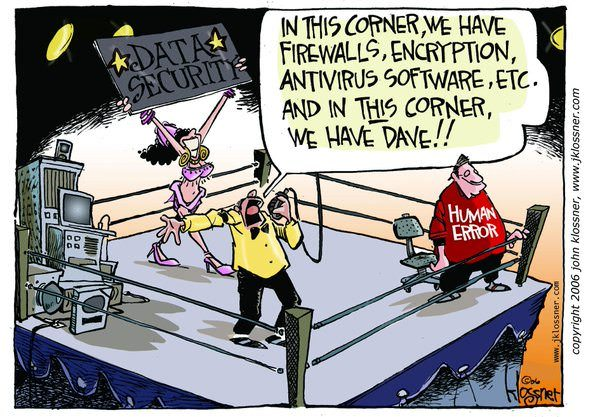
\includegraphics[width=.7\textwidth]{DaveSecurity}
\caption{Network Security - the sad truth}
\label{fig:dave}
\end{center}
\end{figure}

Note that, likewise tables and listings, you shall not worry about where the figures are placed. Moreover, you should not add the file extension (LaTeX will pick the `best' one for you) or the figure path.
